% JIKI manuscript -- LaTeX version of the paper "Explainable Federated Detection of
% Six-Class Oil Palm Fresh Fruit Bunch Ripeness: A Grad-CAM++ Faithfulness Study for
% Harvest Decision Support" (Jurnal Ilmu Komputer dan Informasi / Journal of Computer
% Science and Information, 15/1 (2022)).
% Build: latexmk -pdf manuscript.tex   -- or open on Overleaf (New Project > Upload Project).
%
% Transcribed from the original PDF (original.pdf in this folder) supplied by the
% author; the two figures already existed as real rendered images in that PDF (not
% placeholders) and were extracted losslessly (pdfimages) rather than redrawn --
% figure1_methodology.png and figure2_gradcam_heatmaps.png.
\documentclass[9pt,twocolumn]{extarticle}

\usepackage[a4paper,top=2.2cm,bottom=2.2cm,left=1.8cm,right=1.8cm,columnsep=0.6cm]{geometry}
\usepackage{mathptmx}
\usepackage[T1]{fontenc}
\usepackage{graphicx}
\usepackage{booktabs}
\usepackage{caption}
\usepackage{amsmath}
\usepackage{xcolor}
\usepackage{fancyhdr}
\usepackage{float}
\usepackage[colorlinks=true,linkcolor=blue,citecolor=blue,urlcolor=blue]{hyperref}
\usepackage[english]{babel}

\newcommand{\todo}[1]{\textcolor{red}{[TODO: #1]}}

% --- Running header, two-sided (mirrors the original PDF's verso/recto headers) ---
\pagestyle{fancy}
\fancyhf{}
\renewcommand{\headrulewidth}{0pt}
\fancyhead[LE]{\small\itshape\thepage\quad Jurnal Ilmu Komputer dan Informasi (Journal of Computer Science and Information), volume 15, issue 1, February 2022}
\fancyhead[RO]{\small\itshape Author et.al. (left it blank for first submission), One Line Article Title\quad\thepage}

\begin{document}

% --- Full-width title block (twocolumn trick) ---
\twocolumn[
  \begin{center}
  \begin{minipage}{0.94\textwidth}
  \centering
    {\small Jurnal Ilmu Komputer dan Informasi (Journal of Computer Science and Information)\par
    15/1 (2022), xx-xx. DOI: \url{http://dx.doi.org/10.21609/jiki.v15i1.xxx}\par}
    \vspace{1.2em}
    {\LARGE\bfseries Explainable Federated Detection of Six-Class Oil Palm Fresh Fruit Bunch Ripeness: A Grad-CAM++ Faithfulness Study for Harvest Decision Support\par}
    \vspace{1em}
    {\large Rachma Dianty$^{1,*}$, Favian Dewanta$^2$, Teddy Surya Gunawan$^3$\par}
    \vspace{0.4em}
    {\small $^{1,2}$Department of Electrical Engineering, School of Electrical Engineering, Telkom University, Bandung, Indonesia\par
    $^3$Department of Electrical and Computer Engineering, International Islamic University Malaysia, Kuala Lumpur 53100, Malaysia\par}
    \vspace{0.4em}
    {\small\itshape Email: rachmadiantyy@gmail.com$^1$, favian@telkomuniversity.ac.id$^2$, tsgunawan@iium.edu.my$^3$\par}
  \end{minipage}
  \end{center}
  \vspace{1em}

  \begin{center}
  \begin{minipage}{0.94\textwidth}
    \small
    \textbf{Abstract}

    Timely harvesting of oil palm fresh fruit bunches (FFB) is decisive for oil yield and quality, yet manual ripeness assessment is subjective and inconsistent. Computer-vision automation promises consistency, but centrally aggregating plantation imagery conflicts with the confidentiality of operational data. This study investigates whether a federated learning (FL) approach, which trains a shared model without moving raw imagery across estates, can deliver six-class FFB ripeness detection that is both accurate and explainable, making it a trustworthy harvest decision-support tool. A YOLOv11n detector is trained federatively using FedAvg over five communication rounds on Non-IID Dirichlet partitions derived from a leakage-free bunch-identity split (training: 9,094 images from 72 bunches; validation: 769 from 8; test: 951 from 9). All BatchNorm layers are converted to GroupNorm for cross-experiment consistency. Explanation quality is assessed with Grad-CAM++ via per-class Average Drop (AD) and Focus Retention Rate (FRR), the latter doubling as an agronomic alignment proxy that measures heatmap intensity within fruit bounding boxes. The federated model attains mAP@0.5 = 0.738, only 0.049 below the centralized reference of 0.787, with global occlusion-based AD = 15.9\% and global FRR = 0.281. Per-class analysis shows that the colour-driven classes (Unripe, Empty Bunch) are the most faithfully localized on the fruit (FRR $\approx$ 0.46), whereas the Abnormal class is the least faithful on both metrics (AD = 7.45\%, FRR = 0.093) and thus warrants manual review. The results indicate that federation can deliver privacy-preserving palm ripeness detection at near-centralized accuracy without sacrificing decision explainability.

    \medskip
    \textbf{Keywords}: explainable artificial intelligence, federated learning, Grad-CAM++, oil palm ripeness, YOLOv11
  \end{minipage}
  \end{center}
  \vspace{1.5em}
]

\section{Introduction}

The oil palm industry is a cornerstone of Indonesian and Malaysian agribusiness, with the two countries together accounting for over 85\% of the world's palm oil supply \cite{usda2024}. At the operational level, the timing of fresh fruit bunch (FFB) harvest is the single most influential decision affecting oil yield and quality. Bunches harvested too early contain insufficient mesocarp oil, whereas bunches harvested too late accumulate Free Fatty Acid (FFA), degrading Crude Palm Oil (CPO) quality. Industry practice distinguishes six commercially relevant ripeness classes, namely \emph{Unripe}, \emph{Underripe}, \emph{Ripe}, \emph{Overripe}, \emph{Empty Bunch}, and \emph{Abnormal} \cite{junos2022}. Traditional assessment by harvest foremen, based on bunch colour and loose fruitlet count, is subjective, with misclassification rates of 15--25\% reported under suboptimal lighting \cite{sabri2017}.

Modern object detectors of the YOLO family \cite{redmon2016}, of which YOLOv11 \cite{khanam2024} is the latest iteration, can localize and classify multiple bunches in a single frame in real time, making vision-based automation feasible at the plantation scale. However, training accurate detectors requires diverse imagery spanning seasons, lighting, and geographic conditions. Centralizing such imagery, however, is impractical: plantation images are commercially sensitive, revealing block locations, production volumes, and operational practices, and estates are therefore reluctant to ship raw data to a shared server.

Federated learning (FL) \cite{mcmahan2017} provides an architectural answer, in which multiple estates collaboratively train a shared model while raw imagery remains on local infrastructure and only model parameters traverse the network. In the taxonomy of Kairouz et al. \cite{kairouz2021}, the plantation-consortium scenario is \emph{cross-silo}, with few clients, each holding large amounts of data, and stable availability.

Accuracy alone, however, is insufficient for field adoption. An agricultural decision-support system must also be trustworthy, because operators need to understand \emph{why} the model labels a bunch as ripe or overripe. Without auditable visual explanations, predictions risk being either rejected outright or trusted uncritically, and both failure modes carry real economic cost. Explainable AI (XAI) methods such as Grad-CAM++ \cite{chattopadhyay2018} generate heatmaps highlighting the image regions most responsible for a prediction, and the quality of such heatmaps can be measured quantitatively through faithfulness metrics.

Distinct from the authors' prior work that characterizes the behaviour of differential privacy on this detector \cite{dianty2026}, the present study addresses an application-oriented question: can federated learning deliver oil palm ripeness detection that is simultaneously accurate and explainable enough to serve as a credible harvest decision-support tool? This paper makes three contributions. First, it presents an in-depth, per-class evaluation of Grad-CAM++ faithfulness on a federated palm ripeness detector, going beyond a single global metric. Second, it introduces a bunch-identity-based anti-leakage split protocol for palm detection datasets. Third, it provides empirical evidence that federation does not significantly degrade the quality of model explanations relative to centralized training.

\section{Literature Review}

\subsection{Vision-Based Oil Palm Ripeness Assessment}

Several studies have investigated automated ripeness assessment using deep learning. Colour-feature classifiers \cite{sabri2017} preceded modern CNN approaches. Junos et al. \cite{junos2022} applied a YOLO variant on UAV imagery for fruit-level detection. More recently, Gunawan et al. \cite{gunawan2023} benchmarked several YOLOv8 variants for FFB ripeness classification, and Elwirehardja et al. \cite{elwirehardja2021} explored lightweight deep-learning models for on-device classification. A common limitation across these works is the assumption of centralized training and the use of only a single mAP number for validation, so that neither the trustworthiness of the visual explanation nor the privacy implications of centralized aggregation is examined. The present work addresses both gaps.

\subsection{Federated Learning for Cross-Silo Scenarios}

McMahan et al. \cite{mcmahan2017} introduced the canonical FedAvg algorithm, in which clients perform local stochastic gradient descent and the server aggregates updates by a data-size-weighted average; a broader survey of FL challenges and methods is given in \cite{li2020fl}. Kairouz et al. \cite{kairouz2021} distinguish \emph{cross-device} settings, with millions of unreliable clients holding little data each, from \emph{cross-silo} settings, with few reliable clients holding large data each; a plantation consortium clearly falls in the latter regime. Data heterogeneity between sites is commonly simulated via Dirichlet partitioning \cite{hsu2019}, where a concentration parameter $\alpha$ controls per-client class imbalance.

\subsection{Explainable AI and Faithfulness Metrics}

Grad-CAM \cite{selvaraju2017} weights each feature-map channel by the spatially-averaged gradient of the target-class score, producing a class activation heatmap. Grad-CAM++ \cite{chattopadhyay2018} refines this using a weighted combination of positive partial derivatives, providing more accurate localization when multiple instances of the same class are present, a condition that routinely occurs in FFB imagery containing several bunches per frame. Two complementary faithfulness metrics are used in this work: Average Drop (AD), which measures the confidence lost when the input is restricted to the heatmap region, and Focus Retention Rate (FRR), which measures the fraction of heatmap intensity falling inside the ground-truth fruit boxes. Both belong to the broader family of perturbation-based faithfulness evaluations such as RISE \cite{petsiuk2018}. In addition, FRR doubles as an agronomic alignment proxy by quantifying whether the heatmap attends to the fruit itself.

\section{Methodology}

Fig.~\ref{fig:methodology} summarizes the end-to-end pipeline of the proposed framework, from dataset acquisition and leakage-free splitting, through Non-IID Dirichlet partitioning and the BatchNorm-to-GroupNorm conversion of the detector, to federated training with FedAvg and per-class Grad-CAM++ faithfulness evaluation. Each phase is detailed below.

\begin{figure*}[t]
  \centering
  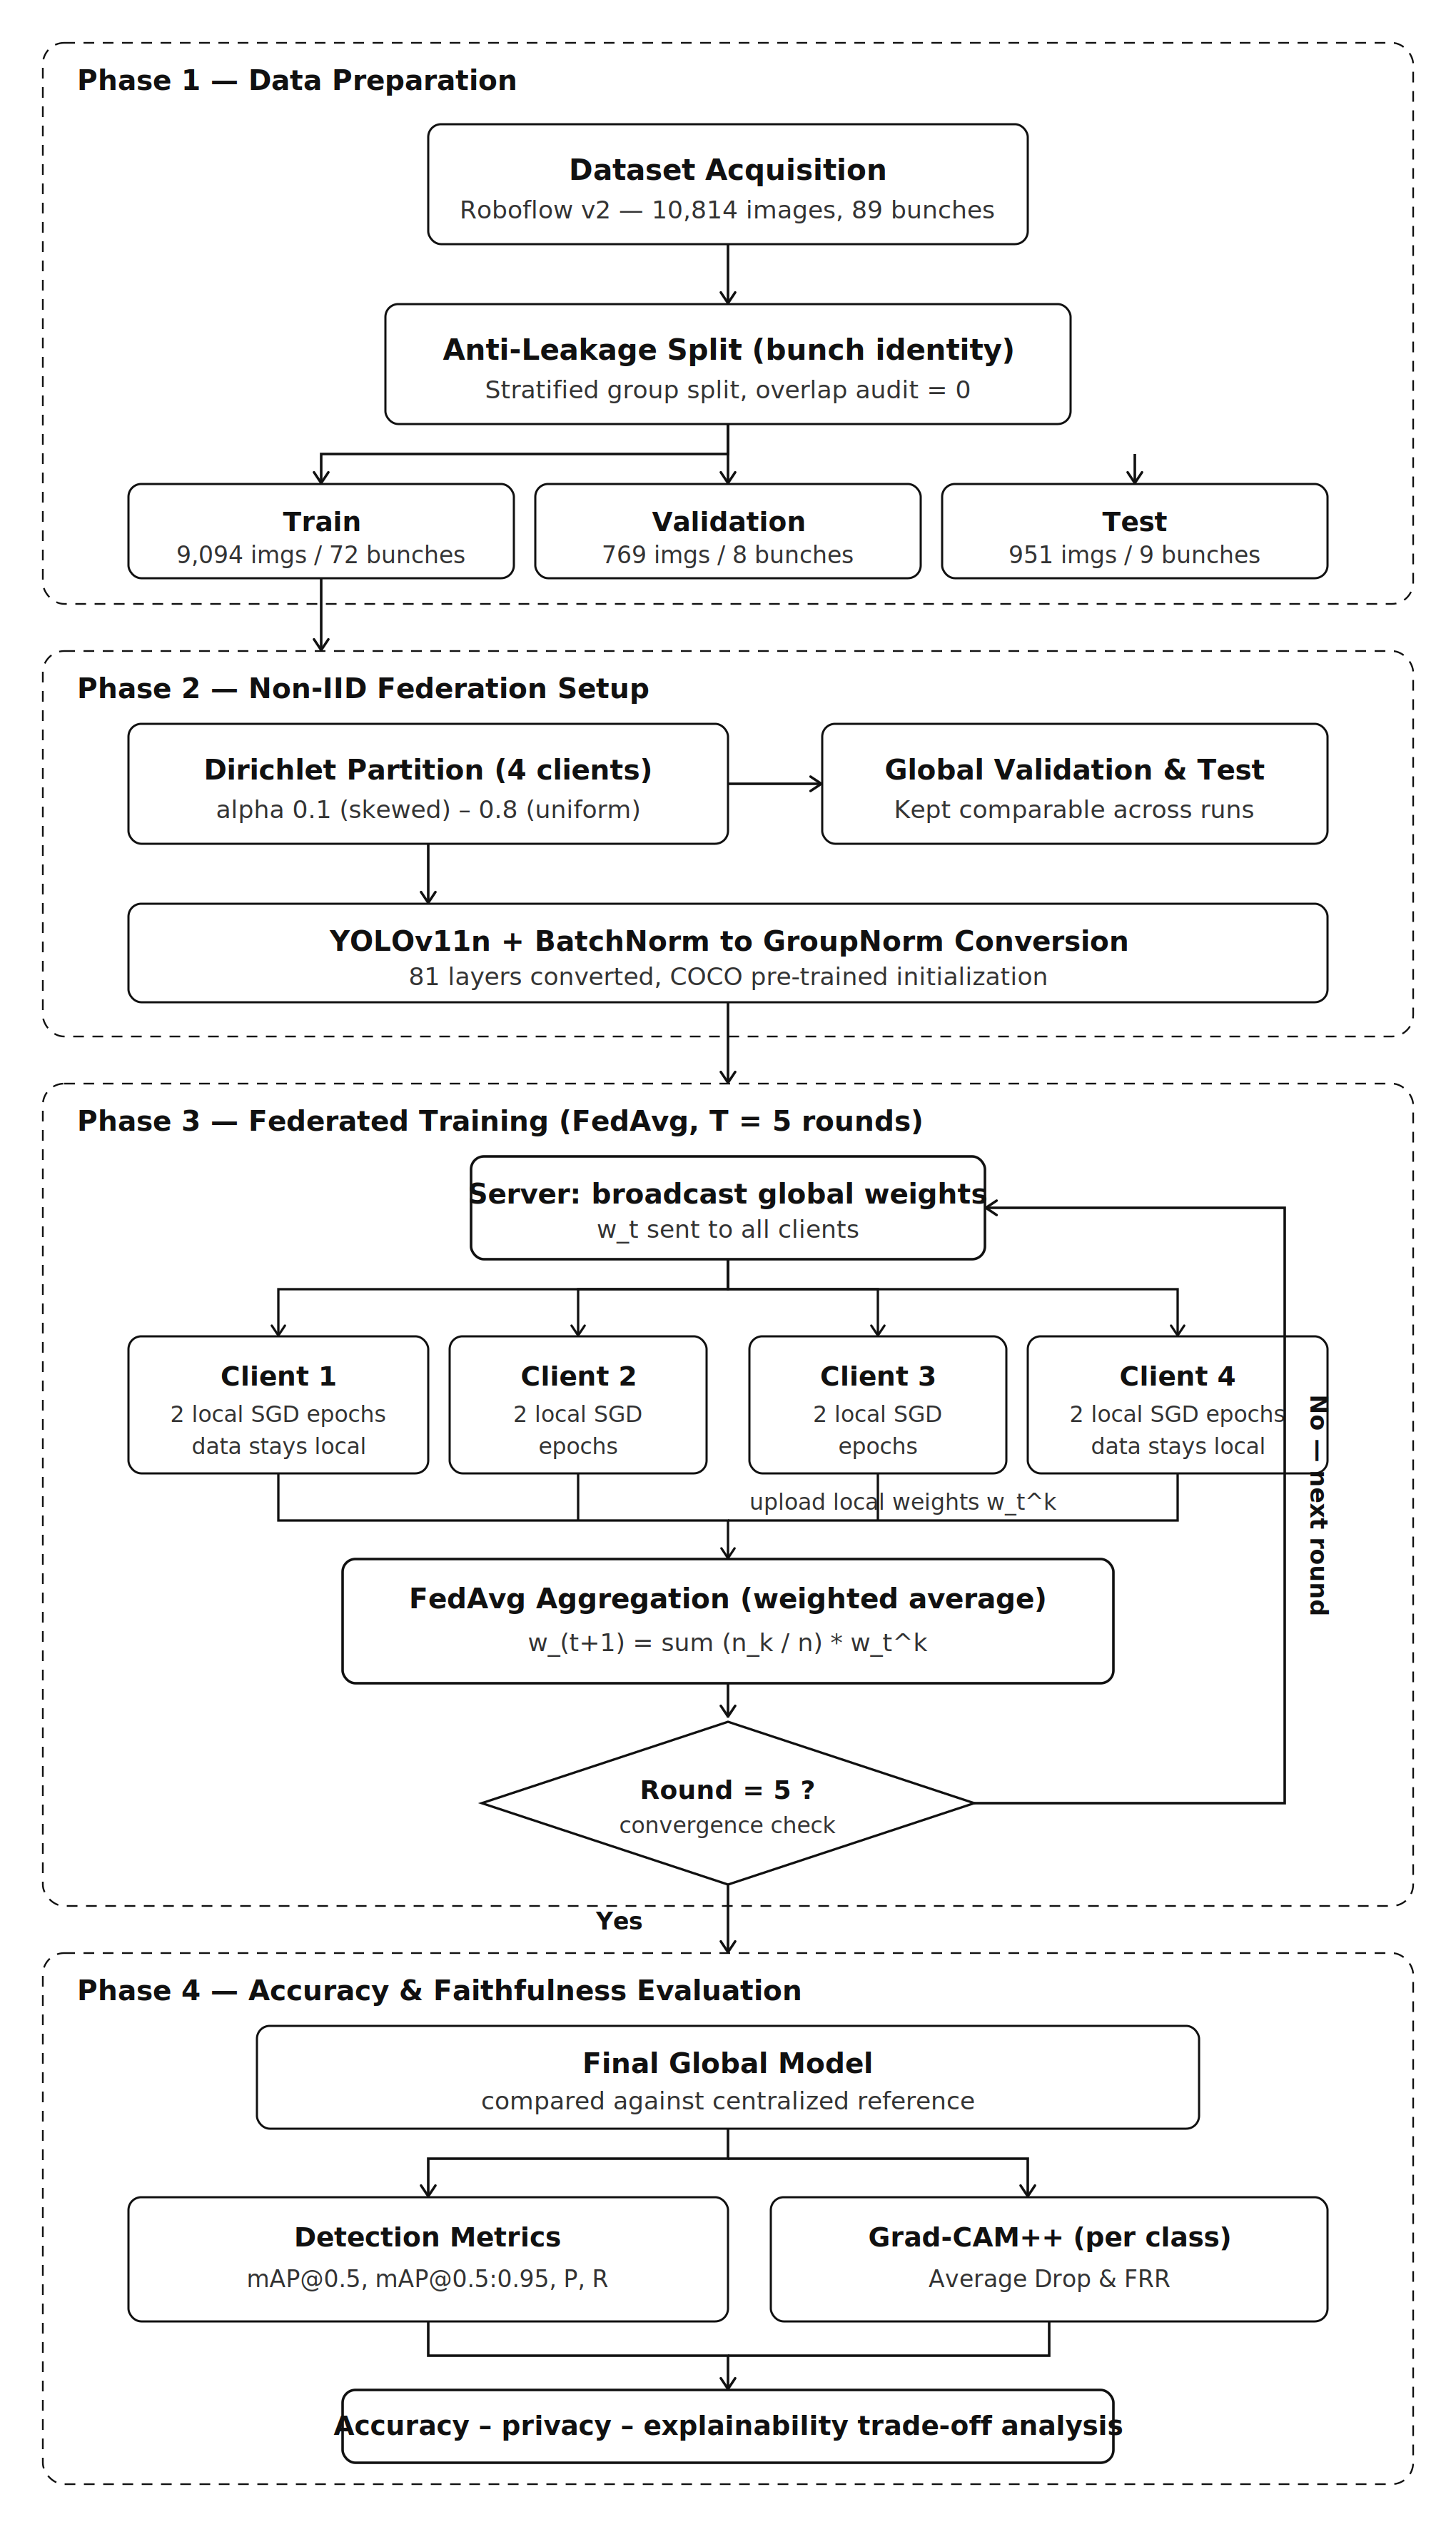
\includegraphics[width=\linewidth]{figure1_methodology.png}
  \caption{Research methodology flow of the proposed federated oil palm ripeness detection framework, from data preparation to Grad-CAM++ faithfulness evaluation.}
  \label{fig:methodology}
\end{figure*}

\subsection{Dataset and Anti-Leakage Split}

The dataset is the palm-fruit-ripeness-detection collection (Roboflow, version 2), comprising 10,814 images from 89 unique bunches, annotated across six classes in alphabetical order: \emph{Abnormal}, \emph{Empty Bunch}, \emph{Overripe}, \emph{Ripe}, \emph{Underripe}, and \emph{Unripe}. A naive random split risks leakage at the bunch level, because multiple frames of the same bunch could be assigned to both training and test partitions, allowing the model to recognize the bunch rather than learn generalizable ripeness cues. To prevent this, a stratified group split keyed by bunch identity is applied, so that each bunch is assigned entirely to one partition, with stratification preserving class balance (Table~\ref{tab:split}). A leakage audit confirmed zero bunch-identity overlap between any two partitions.

\begin{table}[H]
  \centering
  \caption{Leakage-free dataset partition by bunch identity.}
  \label{tab:split}
  \small
  \begin{tabular}{lrr}
    \toprule
    Partition & Images & Unique bunches \\
    \midrule
    Train & 9,094 & 72 \\
    Validation & 769 & 8 \\
    Test (held out) & 951 & 9 \\
    \midrule
    \textbf{Total} & \textbf{10,814} & \textbf{89} \\
    \bottomrule
  \end{tabular}
\end{table}

\subsection{Non-IID Federation Setup}

The training partition is divided among $K=4$ clients using a Dirichlet distribution with per-client concentration parameters spanning $\alpha=0.1$ (highly skewed) to $\alpha=0.8$ (near uniform), simulating realistic heterogeneity across estates. Validation and test partitions are kept global so that metrics are directly comparable across configurations.

\subsection{Detector and Architectural Modification}

The base detector is YOLOv11n, with approximately 2.6 million parameters, initialized from COCO \cite{lin2014} pre-trained weights. All 81 Batch Normalization (BatchNorm) layers are converted in place to Group Normalization (GroupNorm) \cite{wu2018}, using eight groups that are auto-reduced when the group count does not divide a layer's channel count, with the affine parameters copied to preserve the pre-trained initialization. This conversion ensures consistency with the companion differential-privacy study \cite{dianty2026}, whose per-sample gradient computation using Differentially Private Stochastic Gradient Descent (DP-SGD) \cite{abadi2016} requires per-sample-independent normalization. After conversion, no BatchNorm layers remain.

\subsection{Federated Training Procedure}

Training uses FedAvg over $T=5$ communication rounds. In each round, every client receives the global parameters $w_t$, performs $E=2$ local epochs of stochastic gradient descent (learning rate 0.01, momentum 0.937, weight decay $5\times10^{-4}$, batch size 16, image size $640\times640$), and returns its updated local parameters $w_t^k$. The server aggregates by data-size weighting, as defined in (1):

\begin{equation}
w_{t+1} = \sum_{k=1}^{K} \frac{n_k}{n} w_t^k
\label{eq:fedavg}
\end{equation}

where $n_k$ is the local shard size of client $k$ and $n=\sum_k n_k$. The loss is the standard YOLOv11 composite of Complete Intersection over Union (CIoU) box loss (weight 7.5), classification loss (weight 0.5), and Distribution Focal Loss (weight 1.5). A centralized reference is trained for 50 epochs on the entire training partition under identical hyperparameters. Formal privacy is treated in detail in the companion paper \cite{dianty2026}; here, privacy is addressed architecturally, since raw imagery never leaves the client, keeping the focus on explainability.

\subsection{Explanation Quality Metrics}

Grad-CAM++ is applied at the last shared convolutional layer before the decoupled detection head, so that class-score gradients propagate through the hooked feature map. Two faithfulness metrics are computed on $N=200$ randomly sampled test images, both globally and per class. We adopt an occlusion-based Average Drop (AD, \%), where higher is better: the most salient region (heatmap value at least 0.5) is replaced with the per-image mean pixel value to occlude it, and AD measures the resulting relative confidence drop, as defined in (2):

\begin{equation}
\text{AD} = \frac{1}{N}\sum_{i=1}^{N} \frac{\max(0,\, Y_i^c - O_i^c)}{Y_i^c} \times 100\%
\label{eq:ad}
\end{equation}

where $Y_i^c$ is the model's confidence on the original image $i$ for class $c$, and $O_i^c$ is its confidence after the salient region is occluded. A large drop means the highlighted region was decisive for the prediction; hence a higher AD indicates a more faithful explanation. Focus Retention Rate (FRR), where higher is better, gives the fraction of heatmap intensity inside the ground-truth boxes, as defined in (3):

\begin{equation}
\text{FRR} = \frac{\sum_{p \in \text{ROI}} I(p)}{\sum_{p \in \text{Image}} I(p)}
\label{eq:frr}
\end{equation}

where $I(p)$ is the heatmap intensity at pixel $p$, and the Region of Interest (ROI) is the union of ground-truth boxes for the target class. FRR thus measures both faithfulness and agronomic alignment, in the sense of whether the model attends to the fruit or to the background.

\section{Results and Discussion}

\subsection{Detection Accuracy}

Table~\ref{tab:accuracy} compares the federated model, trained with four Non-IID clients, against the centralized reference. The federated detector reaches mAP@0.5 = 0.738, only 0.049 (about 6\%) below the centralized upper bound of 0.787, which is a small utility cost given that no raw imagery is ever shared. Both models sit in the acceptable range ($\geq 0.70$), indicating that communication-constrained federation remains a viable basis for harvest decision support.

\begin{table}[H]
  \centering
  \caption{Detection performance on the held-out test set. FL cost is computed as centralized minus federated.}
  \label{tab:accuracy}
  \small
  \begin{tabular}{lrrrr}
    \toprule
    Model & mAP@0.5 & mAP@.5:.95 & Prec. & Rec. \\
    \midrule
    Centralized (reference) & 0.787 & 0.672 & 0.815 & 0.833 \\
    Federated (FedAvg, K=4) & 0.738 & 0.584 & 0.626 & 0.727 \\
    \midrule
    \textbf{FL cost (absolute)} & \textbf{0.049} & \textbf{0.088} & \textbf{0.189} & \textbf{0.106} \\
    \bottomrule
  \end{tabular}
\end{table}

\subsection{Per-Class Faithfulness}

Table~\ref{tab:perclass} reports AD and FRR per ripeness class plus the global average over 344 class-instances across 200 images. The two metrics agree on the extremes. The \emph{Unripe} and \emph{Empty Bunch} classes exhibit the highest FRR ($\approx 0.46$), meaning that their heatmaps are the most tightly localized on the fruit, whereas the \emph{Ripe} and \emph{Underripe} classes show the highest occlusion sensitivity (AD $\approx 26\%$), meaning that the highlighted region is the most decisive for those predictions. The clearly weakest class on both metrics is \emph{Abnormal} (AD = 7.45\%, FRR = 0.093), since occluding the salient region barely changes the prediction and most heatmap intensity falls outside the fruit boxes. This is agronomically plausible, because \emph{Abnormal} bunches lack a single consistent localized cue and exhibit high intra-class visual variation, so the model's attention disperses onto the background. Operationally, \emph{Abnormal} predictions therefore warrant manual confirmation, whereas the colour-driven ripeness classes can be trusted with higher automation confidence.

This breakdown carries direct operational value, because estates can calibrate operator review effort by ripeness class. A single global number would have obscured this distinction.

\begin{table}[H]
  \centering
  \caption{Per-class Grad-CAM++ faithfulness on the federated model. AD (occlusion-based) is higher-is-better in percent, FRR is higher-is-better on a 0--1 scale, and $n$ is the number of class-instances scored.}
  \label{tab:perclass}
  \small
  \begin{tabular}{lrrr}
    \toprule
    Class & $n$ & AD (\%) & FRR \\
    \midrule
    Abnormal & 72 & 7.45 & 0.093 \\
    Empty Bunch & 20 & 20.90 & 0.462 \\
    Overripe & 45 & 18.93 & 0.343 \\
    Ripe & 124 & 26.29 & 0.292 \\
    Underripe & 49 & 26.68 & 0.270 \\
    Unripe & 34 & 15.71 & 0.463 \\
    \midrule
    \textbf{Global} & \textbf{344} & \textbf{15.90} & \textbf{0.281} \\
    \bottomrule
  \end{tabular}
\end{table}

\subsection{Effect of Federation on Explanation Quality}

To isolate whether federation itself harms explanation quality, the identical Grad-CAM++ protocol was applied to the centralized reference model on the same 200 test images. As Table~\ref{tab:fedvscentral} shows, the federated model is not degraded relative to the centralized one: its global occlusion-based AD is 15.9\% versus 4.95\%, and its global FRR is 0.281 versus 0.182. The higher federated AD means that its predictions depend more decisively on a localized region, and the higher FRR means that this region lies more often on the fruit; that is, federation yields more spatially concentrated and fruit-aligned explanations in this setting. Crucially, both training regimes agree on the hardest case: \emph{Abnormal} has the lowest FRR under either regime (0.093 federated, 0.078 centralized), confirming that this difficulty is intrinsic to the class rather than an artefact of federation. We therefore find no evidence that communication-constrained federation compromises explanation faithfulness, which supports the practical adoption of FL where raw-data sharing is constrained.

\begin{table}[H]
  \centering
  \caption{Global Grad-CAM++ faithfulness, comparing the centralized reference against the federated model on the same test images. Federation does not degrade explanation quality.}
  \label{tab:fedvscentral}
  \small
  \begin{tabular}{lrr}
    \toprule
    Global metric & Centralized & Federated \\
    \midrule
    AD (\%), higher better & 4.95 & 15.90 \\
    FRR (0--1), higher better & 0.182 & 0.281 \\
    \bottomrule
  \end{tabular}
\end{table}

\subsection{Qualitative Analysis}

Fig.~\ref{fig:heatmaps} shows representative Grad-CAM++ heatmaps, one per ripeness class. The qualitative maps corroborate the quantitative findings: for the colour-driven classes such as \emph{Unripe} and \emph{Empty Bunch}, the high-intensity region concentrates on the fruit surface, mirroring their high FRR, whereas for the \emph{Abnormal} class, the activation is comparatively diffuse and partly spills onto the surrounding canopy, consistent with its low FRR and AD.

\begin{figure*}[t]
  \centering
  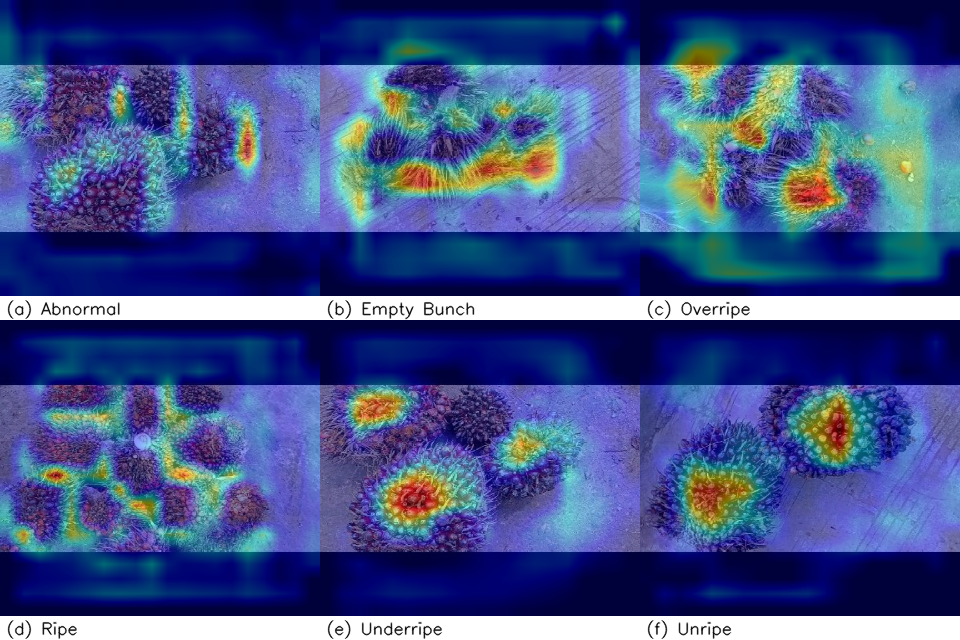
\includegraphics[width=\linewidth]{figure2_gradcam_heatmaps.png}
  \caption{Representative Grad-CAM++ heatmaps for the six ripeness classes. Highlight intensity, where red is high, indicates the image regions most influential to the per-class prediction.}
  \label{fig:heatmaps}
\end{figure*}

\subsection{Threats to Validity}

A single dataset source bounds generalization, and multi-estate validation is left to future work. Heatmap faithfulness is one operational measure of trustworthiness, and complementary user studies with harvest foremen would strengthen the agronomic claim. FRR rewards heatmaps concentrated inside the ground-truth boxes, which may under-credit explanations that correctly attend to nearby cues such as fallen fruitlets; the per-class AD provides a complementary signal that compensates for this limitation.

\section{Conclusion}

This paper investigated whether federated learning can deliver six-class oil palm ripeness detection that is simultaneously accurate and explainable enough to serve as a trustworthy harvest decision-support tool. On a leakage-free bunch-identity split, a federated YOLOv11n--GroupNorm detector trained with FedAvg attains mAP@0.5 = 0.738, only 0.049 (about 6\%) below the centralized reference (0.787). The per-class Grad-CAM++ evaluation yields global AD = 15.9\% and global FRR = 0.281, with the colour-driven ripeness classes the most faithfully explained and the \emph{Abnormal} class the least faithful on both metrics, indicating where human oversight remains necessary. These results support the practical viability of privacy-preserving collaborative training for plantation consortia, where near-centralized accuracy is retained without sharing raw imagery and model decisions remain visually auditable. Future work includes integration of per-sample differential privacy \cite{dianty2026}, multi-estate validation across cultivars and climates, and edge-deployment benchmarks for in-field inference.

\section*{CRediT Authorship Contribution Statement}

\textbf{R. Dianty:} Conceptualization, Methodology, Software, Validation, Writing -- Original Draft, Writing -- Review \& Editing, Visualization. \textbf{F. Dewanta:} Formal analysis, Data Curation, Writing -- Original Draft, Supervision. \textbf{T. S. Gunawan:} Investigation, Writing -- Review \& Editing, Supervision, Project Administration.

\section*{Declaration of Competing Interest}

The authors declare that they have no known competing financial interests or personal relationships that could have appeared to influence the work reported in this paper.

\section*{Declaration of Generative AI and AI-assisted Technologies in the Writing Process}

The authors used Claude (Anthropic) to assist with drafting and improving the writing clarity of this paper and with LaTeX formatting. All experimental design, code, results, and analysis are the authors' own. The authors reviewed and edited the AI-assisted content and take full responsibility for the final publication.

\section*{Data Availability}

The dataset analyzed in this study is openly available from Roboflow (palm-fruit-ripeness-detection, version 2). The leakage-free bunch-identity split protocol and partition lists used in this study are available from the corresponding author upon reasonable request.

\begin{thebibliography}{99}

\bibitem{usda2024} USDA Foreign Agricultural Service, ``Oilseeds: World markets and trade,'' USDA, Washington, DC, Tech. Rep., 2024.

\bibitem{junos2022} M. H. Junos, A. S. Mohd Khairuddin, S. Thannirmalai, and M. Dahari, ``Automatic detection of oil palm fruits from UAV images using an improved YOLO model,'' \emph{The Visual Computer}, vol. 38, pp. 2341--2355, 2022.

\bibitem{sabri2017} N. Sabri, Z. Ibrahim, S. Syahlan, N. Jamil, and N. N. A. Mangshor, ``Palm oil fresh fruit bunch ripeness grading identification using color features,'' \emph{Journal of Fundamental and Applied Sciences}, vol. 9, no. 4S, 2017.

\bibitem{redmon2016} J. Redmon, S. Divvala, R. Girshick, and A. Farhadi, ``You only look once: Unified, real-time object detection,'' in \emph{Proc. IEEE Conf. on Computer Vision and Pattern Recognition (CVPR)}, 2016, pp. 779--788.

\bibitem{khanam2024} R. Khanam and M. Hussain, ``YOLOv11: An overview of the key architectural enhancements,'' arXiv preprint arXiv:2410.17725, 2024.

\bibitem{mcmahan2017} B. McMahan, E. Moore, D. Ramage, S. Hampson, and B. A. y Arcas, ``Communication-efficient learning of deep networks from decentralized data,'' in \emph{Proc. 20th Int. Conf. on Artificial Intelligence and Statistics (AISTATS)}, 2017, pp. 1273--1282.

\bibitem{kairouz2021} P. Kairouz, H. B. McMahan, \emph{et al.}, ``Advances and open problems in federated learning,'' \emph{Foundations and Trends in Machine Learning}, vol. 14, no. 1--2, pp. 1--210, 2021.

\bibitem{chattopadhyay2018} A. Chattopadhyay, A. Sarkar, P. Howlader, and V. N. Balasubramanian, ``Grad-CAM++: Generalized gradient-based visual explanations for deep convolutional networks,'' in \emph{Proc. IEEE Winter Conf. on Applications of Computer Vision (WACV)}, 2018, pp. 839--847.

\bibitem{gunawan2023} T. S. Gunawan, M. Kartiwi, H. Mansor, and N. M. Yusoff, ``Palm fruit ripeness detection and classification using various YOLOv8 models,'' in \emph{2023 IEEE 9th Int. Conf. on Smart Instrumentation, Measurement and Applications (ICSIMA)}, 2023, pp. 193--198.

\bibitem{elwirehardja2021} G. N. Elwirehardja, J. S. Prayoga, \emph{et al.}, ``Oil palm fresh fruit bunch ripeness classification on mobile devices using deep learning approaches,'' \emph{Computers and Electronics in Agriculture}, vol. 188, p. 106359, 2021.

\bibitem{li2020fl} T. Li, A. K. Sahu, A. Talwalkar, and V. Smith, ``Federated learning: Challenges, methods, and future directions,'' \emph{IEEE Signal Processing Magazine}, vol. 37, no. 3, pp. 50--60, 2020.

\bibitem{hsu2019} T.-M. H. Hsu, H. Qi, and M. Brown, ``Measuring the effects of non-identical data distribution for federated visual classification,'' arXiv preprint arXiv:1909.06335, 2019.

\bibitem{selvaraju2017} R. R. Selvaraju, M. Cogswell, A. Das, R. Vedantam, D. Parikh, and D. Batra, ``Grad-CAM: Visual explanations from deep networks via gradient-based localization,'' in \emph{Proc. IEEE Int. Conf. on Computer Vision (ICCV)}, 2017, pp. 618--626.

\bibitem{petsiuk2018} V. Petsiuk, A. Das, and K. Saenko, ``RISE: Randomized input sampling for explanation of black-box models,'' in \emph{British Machine Vision Conference (BMVC)}, 2018.

\bibitem{dianty2026} R. Dianty \emph{et al.}, ``FedX-Palm: Per-sample DP-SGD versus client-level DP-FedAvg for privacy-preserving oil palm ripeness detection on YOLOv11,'' 2026.

\bibitem{lin2014} T.-Y. Lin \emph{et al.}, ``Microsoft COCO: Common objects in context,'' in \emph{European Conference on Computer Vision (ECCV)}, 2014, pp. 740--755.

\bibitem{wu2018} Y. Wu and K. He, ``Group normalization,'' in \emph{European Conference on Computer Vision (ECCV)}, 2018, pp. 3--19.

\bibitem{abadi2016} M. Abadi \emph{et al.}, ``Deep learning with differential privacy,'' in \emph{Proc. ACM SIGSAC Conf. on Computer and Communications Security (CCS)}, 2016, pp. 308--318.

\end{thebibliography}

\end{document}
